%%% CSE 4316 ADS - WORKED EXAMPLE (Autonomous Ground Robot)
%%% Structure follows ISO/IEC/IEEE 42010:2022 + IEEE 1016-2009.
\documentclass[11pt,letterpaper]{article}
\usepackage[margin=1.0in]{geometry}
\usepackage[T1]{fontenc}
\usepackage[bitstream-charter]{mathdesign}
\usepackage[latin1]{inputenc}
\usepackage{amsmath}\usepackage{xcolor}\usepackage{cite}\usepackage{hyphenat}
\usepackage{graphicx}\usepackage{float}\usepackage{subfigure}\usepackage{sectsty}
\usepackage[compact]{titlesec}\usepackage[tablegrid]{vhistory}\usepackage{pbox}\usepackage{longtable}
\usepackage{tikz}\usetikzlibrary{positioning,arrows.meta,fit,backgrounds}
\allsectionsfont{\color{accentcolor}\scshape\selectfont}
\definecolor{accentcolor}{rgb}{0.0,0.0,0.5}
% --- shared diagram styles (module boxes carry real subsystem names) ---
\tikzset{
  mod/.style={draw, rounded corners, fill=white, minimum height=8mm, minimum width=27mm, font=\footnotesize, align=center, inner sep=2pt},
  ext/.style={draw, dashed, rounded corners, fill=black!4, minimum height=8mm, minimum width=24mm, font=\footnotesize\itshape, align=center, inner sep=2pt},
  band/.style={draw=accentcolor!45, rounded corners, inner sep=3.5mm},
  llbl/.style={font=\small\bfseries, text=accentcolor, align=left},
  flow/.style={-{Latex[length=2mm]}, thick, draw=accentcolor!80},
  fl/.style={font=\scriptsize, fill=white, inner sep=1pt},
}
\newcommand{\teamname}{Team Trailblazer}
\newcommand{\productname}{TerraScout Autonomous Ground Rover}
\newcommand{\coursename}{CSE 4316: Senior Design I}
\newcommand{\semester}{Fall 2026}
\newcommand{\docname}{Architectural Design Specification}
\newcommand{\department}{Department of Computer Science \& Engineering}
\newcommand{\university}{The University of Texas at Arlington}
\newcommand{\authors}{Alan Turing \\ Grace Hopper \\ John Von Neumann \\ Ada Lovelace \\ Charles Babbage}
\usepackage{fancyhdr}\pagestyle{fancy}\usepackage{lastpage}
\lhead{}\chead{}\rhead{}\lfoot{\footnotesize \teamname \ - \semester}\cfoot{}
\rfoot{\footnotesize page \thepage\ of \pageref{LastPage}}
\renewcommand{\headrulewidth}{0.0pt}\renewcommand{\footrulewidth}{0.4pt}
\usepackage[runin]{abstract}\abslabeldelim{\quad}\setlength{\abstitleskip}{-10pt}
\renewcommand{\abstractname}{}\renewcommand{\abstracttextfont}{\color{accentcolor} \small \slshape}

\begin{document}
{\centering \huge \color{accentcolor} \sc \textbf{\department \\ \university} \par}
\vspace{1 in}
{\centering \huge \color{accentcolor} \sc \textbf{\docname \\ \coursename \\ \semester} \par}
\vspace{0.5 in}
\begin{figure}[h!]\centering
\includegraphics[width=0.60\textwidth]{images/test_image}\end{figure}
\vspace{0.5 in}
{\centering \huge \color{accentcolor} \sc \textbf{\teamname \\ \productname} \par}
\vspace{0.5 in}
{\centering \large \sc \textbf{\authors} \par}
\newpage

\begin{versionhistory}
  \vhEntry{0.1}{11.02.2026}{JVN}{document creation}
  \vhEntry{1.0}{11.18.2026}{AT|GH|CB}{official release}
\end{versionhistory}
\newpage
\setcounter{tocdepth}{2}\tableofcontents
\newpage

\section{Introduction}
This ADS describes the architecture of \productname\ as an architecture description
per ISO/IEC/IEEE 42010:2022 \cite{ISO42010}, using design viewpoints from IEEE Std
1016-2009 \cite{IEEE1016}. It refines the requirements baselined in the SRS and the
concept in the Project Charter. Scope: the rover, its ground-station link, and its
charging dock.

\section{Stakeholders \& Architectural Concerns}
\begin{table}[H]\begin{center}
\begin{tabular}{ | p{3.5cm} | p{9.5cm} |}\hline
\textbf{Stakeholder} & \textbf{Primary concerns} \\ \hline
Sponsor (O\&M) & inspection coverage, fault-detection quality, cost, safety \\ \hline
Field technician & simple operation, reliability, safe behavior near people \\ \hline
Development team & feasibility, modularity, testability, integration risk \\ \hline
Maintainers & diagnosability, replaceable detection model, documentation \\ \hline
Instructor/safety & compliance with lab and robot-safety policy \\ \hline
\end{tabular}\end{center}\end{table}

\section{Architecture Viewpoints}
\begin{table}[H]\begin{center}
\begin{tabular}{ | p{3cm} | p{6.5cm} | p{3cm} |}\hline
\textbf{Viewpoint} & \textbf{Frames} & \textbf{Realized in} \\ \hline
Context & boundary, external actors & Section 4 \\ \hline
Composition/Data Flow & layer/subsystem decomposition, data & Section 5 \\ \hline
Logical/Functional & subsystem responsibilities \& interfaces & Sections 6--8 \\ \hline
Deployment & software-to-hardware mapping & Section 8 \\ \hline
\end{tabular}\end{center}\end{table}
\subsection{Architectural Style \& Conventions}
The system uses a three-layer robotics stack: \textbf{Perception \& Sensing},
\textbf{Autonomy \& Compute}, and \textbf{Mobility \& Power}. Subsystems
communicate over a ROS~2 message bus on the compute module; hardware interfaces use
USB, CSI, and CAN. Interface identifiers use \texttt{\#NN}. Layers are named by
function; subsystems are named \texttt{[Layer].[Name]}.

\section{System Overview \& Context View}
\begin{figure}[h!]\centering
\resizebox{0.95\textwidth}{!}{%
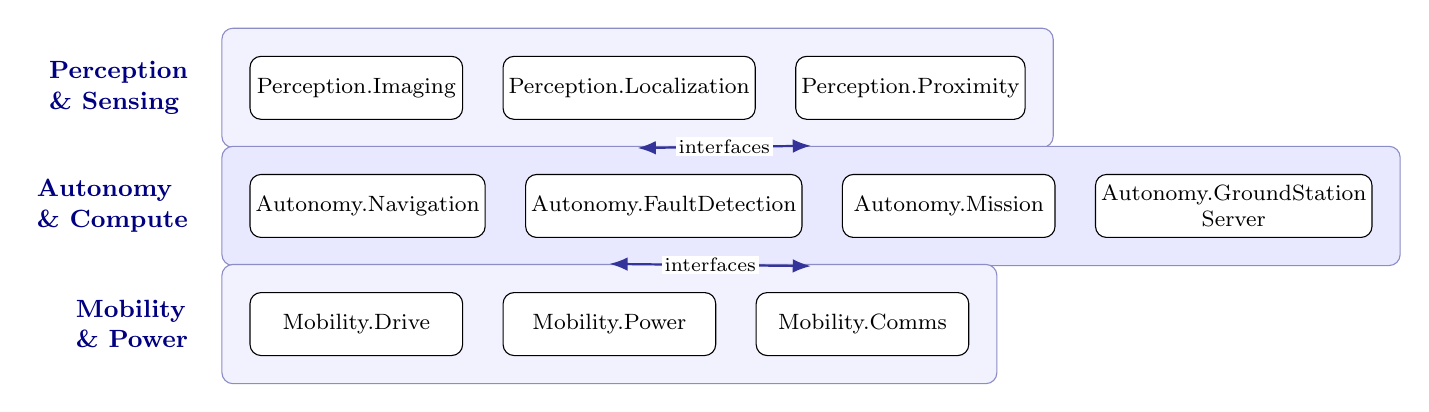
\begin{tikzpicture}[node distance=5mm]
\node[mod] (ximg) {Perception.Imaging};
\node[mod, right=of ximg] (xloc) {Perception.Localization};
\node[mod, right=of xloc] (xprox) {Perception.Proximity};
\node[mod, below=15mm of ximg.west, anchor=west] (ynav) {Autonomy.Navigation};
\node[mod, right=of ynav] (yfd) {Autonomy.FaultDetection};
\node[mod, right=of yfd] (ymis) {Autonomy.Mission};
\node[mod, right=of ymis] (ygs) {Autonomy.GroundStation\\Server};
\node[mod, below=15mm of ynav.west, anchor=west] (zdrv) {Mobility.Drive};
\node[mod, right=of zdrv] (zpow) {Mobility.Power};
\node[mod, right=of zpow] (zcom) {Mobility.Comms};
\begin{scope}[on background layer]
\node[band, fill=blue!5,  fit=(ximg)(xprox)] (bx) {};
\node[band, fill=blue!9,  fit=(ynav)(ygs)]  (by) {};
\node[band, fill=blue!5,  fit=(zdrv)(zcom)] (bz) {};
\end{scope}
\node[llbl, left=3mm of bx] {Perception\\\& Sensing};
\node[llbl, left=3mm of by] {Autonomy\\\& Compute};
\node[llbl, left=3mm of bz] {Mobility\\\& Power};
\draw[{Latex}-{Latex}, thick, draw=accentcolor!80] (bx.south) -- (by.north) node[fl,midway]{interfaces};
\draw[{Latex}-{Latex}, thick, draw=accentcolor!80] (by.south) -- (bz.north) node[fl,midway]{interfaces};
\end{tikzpicture}}
\caption{Three-layer architecture of the rover, showing each layer's subsystems}\end{figure}
External actors: the operator (via the ground-station web page and WebSocket link),
the physical PV field (sensed environment), and the charging dock (docking + power).
The Perception layer converts the physical world into data; the Autonomy layer turns data into
decisions and reports; the Mobility layer turns decisions into motion and manages power.

\section{Subsystem Definitions \& Data Flow}
\begin{figure}[h!]\centering
\resizebox{\textwidth}{!}{%
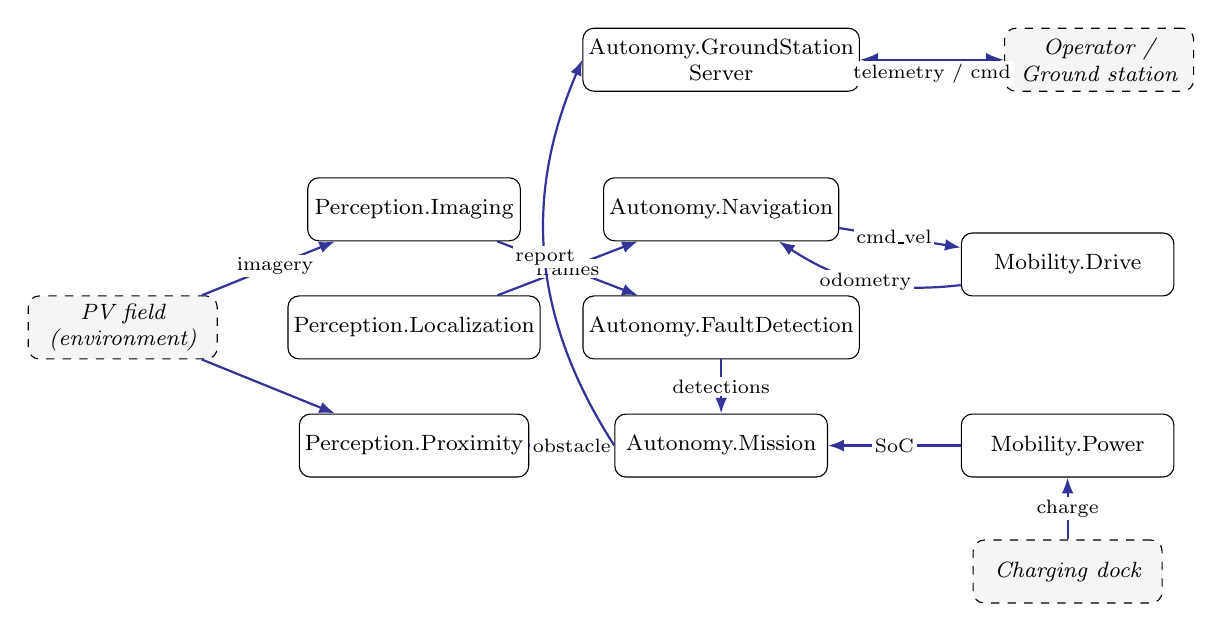
\begin{tikzpicture}
\node[ext] (env) at (0,0) {PV field\\(environment)};
\node[mod] (ximg) at (3.7,1.5) {Perception.Imaging};
\node[mod] (xloc) at (3.7,0)   {Perception.Localization};
\node[mod] (xprox) at (3.7,-1.5){Perception.Proximity};
\node[mod] (ynav) at (7.6,1.5) {Autonomy.Navigation};
\node[mod] (yfd)  at (7.6,0)   {Autonomy.FaultDetection};
\node[mod] (ymis) at (7.6,-1.5){Autonomy.Mission};
\node[mod] (ygs)  at (7.6,3.4) {Autonomy.GroundStation\\Server};
\node[mod] (zdrv) at (12.0,0.8){Mobility.Drive};
\node[mod] (zpow) at (12.0,-1.5){Mobility.Power};
\node[ext] (gs)   at (12.4,3.4){Operator /\\Ground station};
\node[ext] (dock) at (12.0,-3.1){Charging dock};
\draw[flow] (env) -- (ximg) node[fl,pos=0.55]{imagery};
\draw[flow] (env) -- (xprox);
\draw[flow] (xloc) -- (ynav) node[fl,pos=0.5]{pose};
\draw[flow] (ximg) -- (yfd) node[fl,pos=0.5]{frames};
\draw[flow] (xprox) -- (ymis) node[fl,pos=0.5]{obstacle};
\draw[flow] (yfd) -- (ymis) node[fl,pos=0.5]{detections};
\draw[flow] (ynav) -- (zdrv) node[fl,pos=0.45]{cmd\_vel};
\draw[flow] (zdrv) to[bend left=20] node[fl,pos=0.5]{odometry} (ynav);
\draw[flow] (zpow) -- (ymis) node[fl,pos=0.5]{SoC};
\draw[flow] (ymis.west) to[bend left=28] node[fl,pos=0.5]{report} (ygs.west);
\draw[{Latex}-{Latex}, thick, draw=accentcolor!80] (ygs.east) -- (gs.west) node[fl,pos=0.5,below]{telemetry / cmd};
\draw[flow] (dock) -- (zpow) node[fl,pos=0.5]{charge};
\end{tikzpicture}}
\caption{Subsystem data flow: sensing $\rightarrow$ autonomy $\rightarrow$ mobility, with the ground station and dock as external actors}\end{figure}
Sensor streams feed localization and perception; the autonomy layer fuses
pose, plans paths, detects faults, and drives the mission state machine, emitting
velocity commands to the platform and status/reports to the ground station.

\section{Perception \& Sensing Layer}
\subsection{Perception.Imaging}
\textbf{Responsibilities:} capture synchronized RGB and thermal frames and tag them
with time and pose. \textbf{Assumptions:} thermal camera provides a USB/CSI stream.
\begin{table}[H]\begin{center}\begin{tabular}{ | p{1cm} | p{6cm} | p{2.6cm} | p{2.6cm} |}\hline
ID & Description & Inputs & Outputs \\ \hline
\#01 & Camera capture bus & trigger, pose stamp & RGB frame, thermal frame \\ \hline
\end{tabular}\end{center}\end{table}
\textbf{Design rationale:} on-camera hardware sync avoids frame-to-pose skew (AD-02).
\subsection{Perception.Localization}
\textbf{Responsibilities:} produce a fused pose from RTK-GNSS and IMU at $\geq$20\,Hz.
\begin{table}[H]\begin{center}\begin{tabular}{ | p{1cm} | p{6cm} | p{2.6cm} | p{2.6cm} |}\hline
ID & Description & Inputs & Outputs \\ \hline
\#02 & Pose estimate & GNSS fix, IMU & fused pose \\ \hline
\end{tabular}\end{center}\end{table}
\subsection{Perception.Proximity}
\textbf{Responsibilities:} detect near obstacles (ultrasonic/bumper) and raise a
stop signal. Feeds FR-05 safe-stop.

\section{Autonomy \& Compute Layer}
\subsection{Autonomy.Navigation}
\textbf{Responsibilities:} plan and follow paths through the waypoint list within
the FR-01 tolerance, avoiding obstacles; emit velocity commands.
\begin{table}[H]\begin{center}\begin{tabular}{ | p{1cm} | p{6cm} | p{2.6cm} | p{2.6cm} |}\hline
ID & Description & Inputs & Outputs \\ \hline
\#03 & Motion command & pose, waypoints, proximity & velocity cmd \\ \hline
\end{tabular}\end{center}\end{table}
\subsection{Autonomy.FaultDetection}
\textbf{Responsibilities:} classify panel regions in captured frames as nominal or
suspected fault (FR-03) and record locations. Model is replaceable (QA-01).
\subsection{Autonomy.Mission}
\textbf{Responsibilities:} run the mission state machine (idle$\rightarrow$patrol
$\rightarrow$capture$\rightarrow$return$\rightarrow$dock), enforce FR-05 triggers,
and assemble the FR-04 report.
\subsection{Autonomy.GroundStationServer}
\textbf{Responsibilities:} terminate the TLS WebSocket (EI-01, SE-01), stream
telemetry, accept commands, and serve reports to the operator page.

\section{Mobility \& Power Layer}
\subsection{Mobility.Drive}
\textbf{Responsibilities:} execute velocity commands via brushless motor controllers
over CAN; enforce E-stop (SA-01) in hardware.
\begin{table}[H]\begin{center}\begin{tabular}{ | p{1cm} | p{6cm} | p{2.6cm} | p{2.6cm} |}\hline
ID & Description & Inputs & Outputs \\ \hline
\#04 & Drive bus (CAN) & velocity cmd & wheel torque, odometry \\ \hline
\end{tabular}\end{center}\end{table}
\subsection{Mobility.Power}
\textbf{Responsibilities:} manage the battery, report state-of-charge (drives FR-05
low-battery), and control dock charging (EI-02).
\subsection{Mobility.Comms}
\textbf{Responsibilities:} provide the Wi-Fi link between the compute module and the
ground station. \textbf{Deployment:} compute module (Autonomy, Perception software)
mounts on the chassis; Mobility subsystems are embedded microcontrollers on the CAN bus.

\section{Architecture Decisions \& Rationale}
\subsection{AD-01: ROS 2 message bus}
\textbf{Context:} multiple concurrent sensing/decision processes. \textbf{Decision:}
adopt ROS~2. \textbf{Alternatives:} custom IPC (more work), ROS~1 (EOL).
\textbf{Consequences:} mature tooling and modularity (supports QA-01) at the cost of
a runtime dependency. \textbf{Affects:} FR-01, FR-03, QA-01.
\subsection{AD-02: On-board (edge) fault detection}
\textbf{Context:} FR-03 plus SE-02 (imagery stays on the private network).
\textbf{Decision:} run detection on-board rather than streaming imagery off-site.
\textbf{Alternatives:} cloud inference (violates SE-02, needs egress).
\textbf{Consequences:} bounded by compute budget; model kept replaceable. \textbf{Affects:} FR-03, SE-02, PE-03.

\section{Requirements Traceability}
\begin{table}[H]\begin{center}\begin{tabular}{ | p{2cm} | p{5.5cm} | p{5cm} |}\hline
\textbf{Req ID} & \textbf{Requirement (abbrev.)} & \textbf{Realizing subsystem(s)} \\ \hline
FR-01 & Waypoint patrol & Autonomy.Navigation, Perception.Localization \\ \hline
FR-02 & Imagery capture & Perception.Imaging \\ \hline
FR-03 & Fault detection & Autonomy.FaultDetection \\ \hline
FR-04 & Inspection report & Autonomy.Mission, Autonomy.GroundStationServer \\ \hline
FR-05 & Safe-stop \& return & Autonomy.Mission, Perception.Proximity, Mobility.Power \\ \hline
SE-01 & Encrypted link & Autonomy.GroundStationServer \\ \hline
SA-01 & Emergency stop & Mobility.Drive \\ \hline
\end{tabular}\end{center}\end{table}

\bibliographystyle{reference/IEEEtran_custom}
\bibliography{reference/refs}{}
\end{document}
